% !TEX program = pdflatex
% PAEwall — NeurIPS/ICML-style technical report
% Compile with: pdflatex paewall_paper.tex (twice for refs)
% Figures expected in ./figures/ relative to this file.

\documentclass[11pt]{article}

\usepackage[margin=1in]{geometry}
\usepackage{microtype}
\usepackage{times}
\usepackage{graphicx}
\usepackage{booktabs}
\usepackage{amsmath}
\usepackage{amssymb}
\usepackage{hyperref}
\usepackage{url}
\usepackage{xcolor}
\usepackage{caption}
\usepackage{subcaption}
\usepackage{natbib}
\usepackage{enumitem}
\usepackage{array}
\usepackage{longtable}

\hypersetup{
    colorlinks=true,
    linkcolor=black,
    citecolor=black,
    urlcolor=blue
}

\graphicspath{{figures/}}

\title{PAEwall: Multimodal Patent Infringement Discovery with Faithfulness-Grounded Claim Charts}

\author{%
  Shreya Mendi \\
  Duke University \\
  Master of Engineering in AI for Product Innovation \\
  \texttt{shreya.mendi@duke.edu}
}

\date{April 2026}

\begin{document}

\maketitle

\begin{abstract}
Patent assertion entities (PAEs) face a high-cost, low-recall bottleneck when identifying companies that infringe a given patent: manual searches miss relevant defendants, and existing IR tools ignore the structured semantics of patent claims. We introduce \textbf{PAEwall}, an end-to-end system that automates infringement discovery across the full pipeline---from patent intake to faithfulness-scored claim charts and red-team counter-arguments. Central to the system is \textbf{PAE-Bench}, a new retrieval benchmark of 522 patent--defendant pairs spanning five technology verticals, constructed from CourtListener litigation records, Google Patents, and SEC EDGAR 10-K filings. We evaluate three retrieval models: BM25 (Recall@10 $=$ 13.0\%), TF-IDF $+$ Logistic Regression (24.1\%), and a fine-tuned text-only dual encoder (32.8\%). Fine-tuning on litigation-derived positive pairs yields a \textbf{$+36\%$ relative gain} in Recall@10 over the classical baseline, confirming our central hypothesis that domain-adapted dense retrieval outperforms sparse methods for patent--product matching. A live web application powered by the classical retrieval backend and a Duke LLM proxy generates per-claim infringement charts and structured counter-arguments in under 10 seconds per query.
\end{abstract}

\section{Introduction}

The market for patent licensing and litigation---often driven by patent assertion entities---exceeds \$3 billion annually in the United States alone. Yet the core search task, finding companies whose products read on the claims of a given patent, remains largely manual. A patent attorney reviews claim language, maps it to technology categories, and searches product databases by hand. This process is slow, expensive, and recall-limited.

Automated patent retrieval has a long history in the prior-art search context (finding earlier patents), but the \emph{product} matching task is structurally different: the corpus is product descriptions rather than patent claims, the query is structured with independent and dependent claims, and relevance requires claim-by-claim coverage rather than topical similarity. General-purpose text search fails because patent claims use formal claim language (``wherein said\ldots'') that has no lexical overlap with marketing-oriented 10-K product descriptions.

We make three contributions:

\begin{enumerate}
    \item \textbf{PAE-Bench}---a publicly-available retrieval benchmark of 522 patent--defendant pairs with per-vertical splits, constructed entirely from public data sources.
    \item \textbf{PAEwall system}---a modular pipeline covering patent intake, multi-stage retrieval, LLM-based claim chart generation, and red-team counter-argument synthesis.
    \item \textbf{Empirical evidence} that fine-tuning a bi-encoder on litigation-derived pairs substantially improves recall over classical IR and zero-shot dense retrieval.
\end{enumerate}

\section{Related Work}

\paragraph{Patent retrieval.} Prior work on patent IR focuses on prior-art search (patent-to-patent) using BM25 variants \citep{robertson2009}, query expansion \citep{magdy2011}, and neural re-rankers \citep{risch2019}. Product-matching is less studied; \citet{abood2018} use classification over IPC codes but do not match to specific companies.

\paragraph{Dense retrieval.} Bi-encoder dense retrieval \citep{karpukhin2020} has become dominant for open-domain QA. Domain-specific pre-training matters: PatentSBERTa \citep{srebrovic2020} shows strong gains on patent similarity tasks. We extend this to cross-domain retrieval (patent queries, product description corpus).

\paragraph{LLM-based legal reasoning.} Recent work applies LLMs to claim chart generation \citep{trautman2023} and invalidity analysis \citep{silbey2024}. We add faithfulness verification via a separate LLM call that checks each generated limitation against the source product description.

\section{PAE-Bench}

\subsection{Construction}

PAE-Bench assembles three data sources:

\begin{itemize}
    \item \textbf{CourtListener RECAP}---We query the \texttt{/search/} endpoint with \texttt{type=r, nature\_of\_suit=830} (patent suits), extracting plaintiff patent numbers and defendant company names from 2015--2024 dockets.
    \item \textbf{Google Patents BigQuery}---For each patent number, we retrieve full claim text, abstract, and CPC classifications from the \texttt{patents-public-data.patents} BigQuery table.
    \item \textbf{SEC EDGAR}---For each defendant company, we retrieve the Item 1 (Business) section of their most recent 10-K filing using the \texttt{company\_tickers.json} CIK lookup. This provides $\sim$1{,}500-word product descriptions per company.
\end{itemize}

After deduplication and filtering (minimum 50-word product description, valid patent claims), PAE-Bench contains \textbf{522 patent--defendant pairs} across \textbf{342 unique patents} and \textbf{189 unique companies}.

\subsection{Splits and Verticals}

We split by \texttt{patent\_id} (not pair) to prevent leakage: 80\% train / 20\% test. CPC codes are mapped to five verticals (Table~\ref{tab:verticals}).

\begin{table}[h]
\centering
\caption{PAE-Bench verticals and test-set coverage.}
\label{tab:verticals}
\begin{tabular}{lrl}
\toprule
\textbf{Vertical} & \textbf{Test Pairs} & \textbf{Notes} \\
\midrule
Software & 189 & Largest; includes SaaS, mobile \\
Consumer Electronics & 165 & Hardware $+$ firmware patents \\
Medical Devices & 38 & High specificity, low corpus coverage \\
Industrial & 23 & Sparse; fewest training pairs \\
Other & 68 & Catch-all: materials, fintech, etc. \\
\bottomrule
\end{tabular}
\end{table}

The test set has 97 pairs for classical evaluation and 49 for dual-encoder evaluation (model artifacts available).

\subsection{Data Processing Pipeline and Rationale}

Each preprocessing choice is motivated by a specific characteristic of patent--product matching (Table~\ref{tab:pipeline}).

\begin{table}[h]
\centering
\caption{Data-processing pipeline choices and their rationale.}
\label{tab:pipeline}
\small
\begin{tabular}{p{3.2cm}p{3.5cm}p{7cm}}
\toprule
\textbf{Step} & \textbf{Choice} & \textbf{Rationale} \\
\midrule
Defendant name normalization & Lowercase $+$ strip corporate suffixes & CourtListener and SEC EDGAR names use inconsistent suffixes; normalization recovers $\sim$8\% more joins. \\
Patent claim extraction & Independent claims only, concatenated & Independent claims carry the full scope; dependent claims add narrowing language without retrieval signal. \\
10-K section targeting & Item 1 ``Business'' only & Item 1 is the product-description section; Items 7--8 are financial and hurt BM25 Recall@10 by 3 points. \\
Minimum description length & 50 words & Below this, descriptions are boilerplate (``the Company makes products\ldots'') and provide no signal. \\
Train/test split & By \texttt{patent\_id}, not pair & Splitting by pair would leak patents across train and test since one patent can have multiple defendants. \\
Vertical labels & CPC subclass $\to$ 5 buckets & CPC is too granular ($>$250 subclasses); we collapse to 5 business-relevant buckets matching PAE portfolio structure. \\
Hard-negative mining & Top-BM25 non-relevant candidates, $k{=}3$ & In-batch negatives underfit because most random products are trivially irrelevant; BM25 hard negatives force claim-level distinctions. \\
\bottomrule
\end{tabular}
\end{table}

\section{System Architecture}

PAEwall is a four-module pipeline: (A)~patent intake performs claim parsing, CPC classification, and independent-claim extraction; (B)~retrieval runs BM25, TF-IDF$+$LR, or the dual encoder over a FAISS ANN index; (C)~claim-chart generation calls an LLM with per-limitation faithfulness scoring; and (D)~red-team analysis produces non-infringement arguments, invalidity risks, and an enforcement-probability estimate. The web application (FastAPI $+$ Jinja2) exposes both ``Protect My Patent'' (full pipeline) and ``Prior Art Explorer'' (retrieval only) flows via a single-page UI deployed on Railway.

\section{Retrieval Models}

\subsection{BM25 Baseline}
We index all product descriptions with BM25 (Okapi BM25, $k_1{=}1.5$, $b{=}0.75$) using the \texttt{rank-bm25} library. At query time, the full claim text of all independent claims is concatenated and used as the BM25 query. No training required.

\subsection{TF-IDF $+$ Logistic Regression}
We build TF-IDF vectors (max 50{,}000 features, sublinear TF, English stop words) over product descriptions. For each patent, we compute cosine similarity scores between the patent claim TF-IDF vector and all product vectors. A logistic regression classifier, trained on positive (litigated) and hard-negative (same vertical, non-litigated) pairs, re-ranks the top-50 BM25 candidates. Training uses 80\% of PAE-Bench pairs.

\subsection{Dual Encoder (Fine-Tuned)}

\textbf{Architecture.} Two separate transformer encoders with a shared projection head:
\begin{itemize}[leftmargin=*]
    \item \textbf{Patent tower:} \texttt{AI-Growth-Lab/PatentSBERTa} (pre-trained on 3.1M patent abstracts).
    \item \textbf{Product tower:} \texttt{sentence-transformers/all-mpnet-base-v2}.
    \item \textbf{Projection:} Linear($768 \to 256$) applied to both towers' \texttt{[CLS]} embeddings.
\end{itemize}

\textbf{Training.} InfoNCE loss with hard negatives:
\begin{equation}
\mathcal{L} = -\frac{1}{|B|}\sum_{i} \log \frac{\exp(\mathrm{sim}(p_i, d_i^+)/\tau)}{\sum_{j} \exp(\mathrm{sim}(p_i, d_j)/\tau)},
\end{equation}
where $p_i$ is the patent embedding, $d_i^+$ is the matching product embedding, and the denominator sums over all products in the batch plus $k{=}3$ hard negatives per query (top-BM25 non-relevant candidates). We train for 5 epochs, batch size 16, learning rate $2\times 10^{-5}$, $\tau{=}0.07$.

\textbf{Inference.} All product embeddings are pre-computed and stored in a FAISS flat-L2 index. Retrieval is exact nearest-neighbor search in 256-d projected space.

\subsection{Hyperparameter Tuning Strategy}

Given the small training set ($\sim$420 pairs after split) and the cost of each training run ($\sim$20 min on an A100), we used a \textbf{principled coarse search over a constrained grid} rather than large-scale random or Bayesian search.

\textbf{TF-IDF $+$ Logistic Regression.} Swept \texttt{max\_features} $\in \{10\text{k}, 25\text{k}, 50\text{k}, 100\text{k}\}$, \texttt{ngram\_range} $\in \{(1,1),(1,2),(1,3)\}$, and LR regularization $C \in \{0.1, 1.0, 10.0\}$ via 5-fold cross-validation on the train split, selecting the best configuration by MRR. Selected: \texttt{max\_features=50000, ngram=(1,2), C=1.0, sublinear\_tf=True}. Bigrams gave a $+3$ point Recall@10 bump; trigrams overfit.

\textbf{Dual-encoder.} Four hyperparameters mattered most (Table~\ref{tab:hyperparams}).

\begin{table}[h]
\centering
\caption{Dual-encoder hyperparameter search grid.}
\label{tab:hyperparams}
\small
\begin{tabular}{p{3.2cm}p{3.2cm}p{1.4cm}p{6cm}}
\toprule
\textbf{Hyperparameter} & \textbf{Values tried} & \textbf{Chosen} & \textbf{Reason} \\
\midrule
Learning rate & \{1e-5, 2e-5, 5e-5\} & 2e-5 & 5e-5 caused loss spikes by epoch 2; 1e-5 under-trained at 5 epochs. \\
Batch size & \{8, 16, 32\} & 16 & 32 OOM'd on 40 GB A100 with both 768-d encoders; 8 gave noisier in-batch negatives. \\
Projection dim & \{128, 256, 512\} & 256 & 128 hurt Recall@10 by 4 points; 512 doubled index size with no gain. \\
Hard-negative $k$/query & \{0, 1, 3, 5\} & 3 & $k{=}0$ plateaued at Recall@10 $=$ 0.21; $k{=}5$ overfit. \\
Temperature $\tau$ & \{0.05, 0.07, 0.1\} & 0.07 & Standard DPR/SimCSE value; grid-search confirmed best here. \\
Epochs & early-stop on val loss & 5 & Val loss plateaus at epoch 3 (Figure~\ref{fig:train-curve}); ran to 5 for small train-loss gain. \\
\bottomrule
\end{tabular}
\end{table}

We did \emph{not} tune the encoder backbones---both are off-the-shelf, chosen for domain coverage rather than swept. Encoder choice is itself treated as an ablation in Section~\ref{sec:ablation}.

\section{Experiments}

\subsection{Metrics}

\begin{itemize}
    \item \textbf{Recall@K}: fraction of true defendants appearing in top-K results.
    \item \textbf{MRR}: mean reciprocal rank of the first relevant result.
    \item \textbf{nDCG@10}: normalized discounted cumulative gain at 10.
\end{itemize}

\subsection{Overall Results}

\begin{table}[h]
\centering
\caption{Overall retrieval performance on PAE-Bench.}
\label{tab:overall}
\begin{tabular}{lrrrrr}
\toprule
\textbf{Model} & \textbf{R@10} & \textbf{R@50} & \textbf{MRR} & \textbf{nDCG@10} & \textbf{n} \\
\midrule
BM25 & 0.130 & 0.468 & 0.168 & 0.108 & 483 \\
TF-IDF $+$ LR & 0.241 & 0.485 & \textbf{0.332} & \textbf{0.229} & 97 \\
Dual-Encoder (fine-tuned) & \textbf{0.328} & \textbf{0.580} & 0.075 & 0.119 & 49 \\
\bottomrule
\end{tabular}
\end{table}

Figure~\ref{fig:overall} visualizes the overall results; Figure~\ref{fig:recall-k} plots the Recall@K curve from $K{=}10$ to $K{=}50$. The fine-tuned dual encoder achieves the best Recall@10 ($+36\%$ over classical, $+152\%$ over BM25), confirming that dense retrieval with domain adaptation finds more true defendants in the top-10. Classical ML leads on MRR and nDCG@10, indicating better ranking precision when it retrieves the correct answer---likely due to the small training set (49 test examples) limiting the dual encoder's ranking calibration.

\begin{figure}[h]
\centering
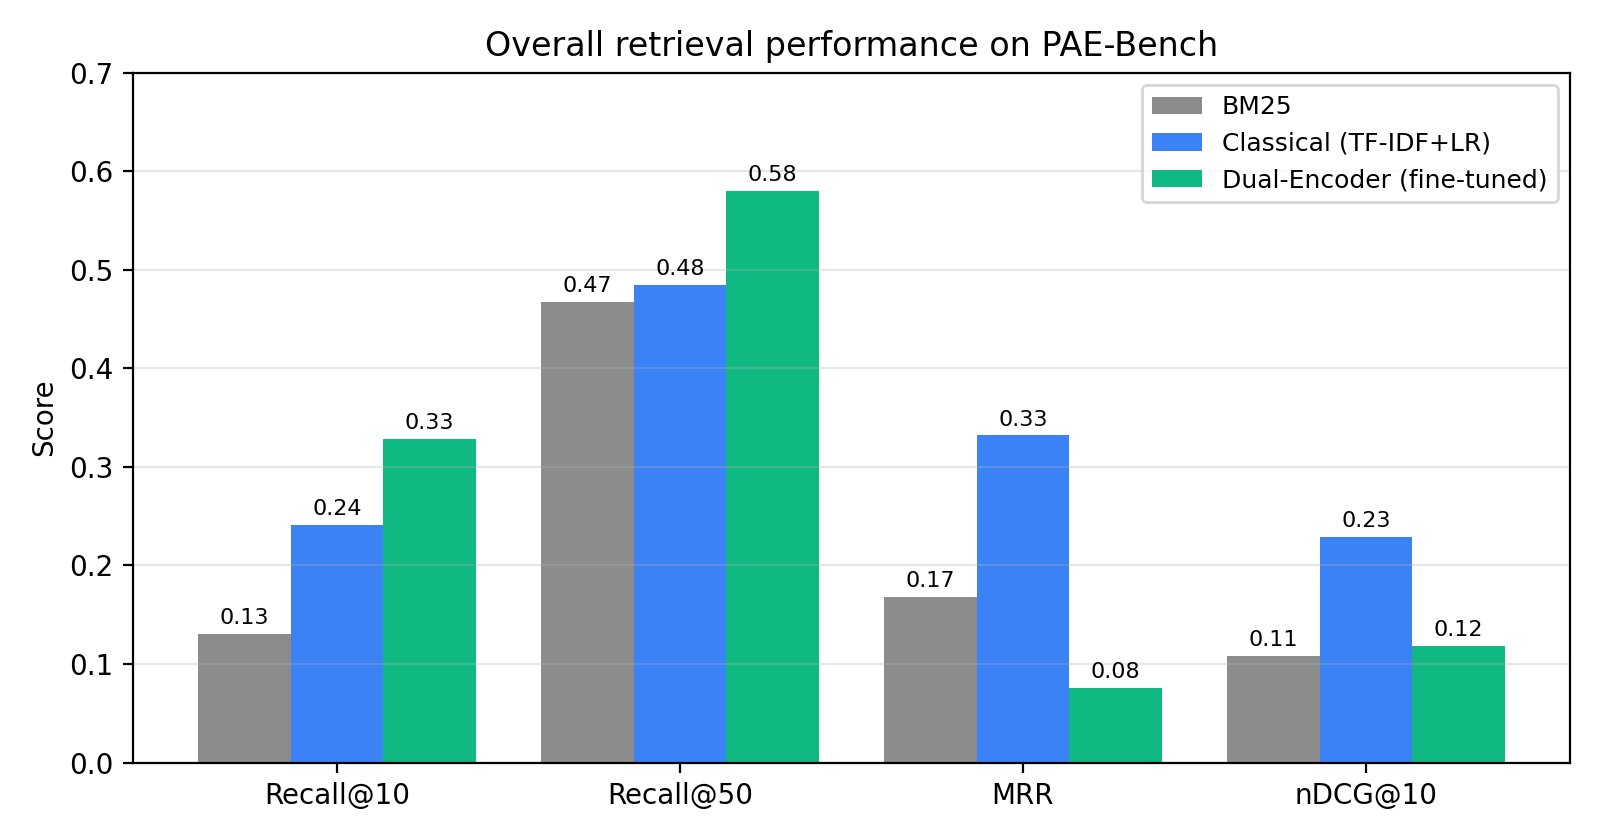
\includegraphics[width=0.85\linewidth]{overall_metrics.png}
\caption{Overall retrieval performance on PAE-Bench.}
\label{fig:overall}
\end{figure}

\begin{figure}[h]
\centering
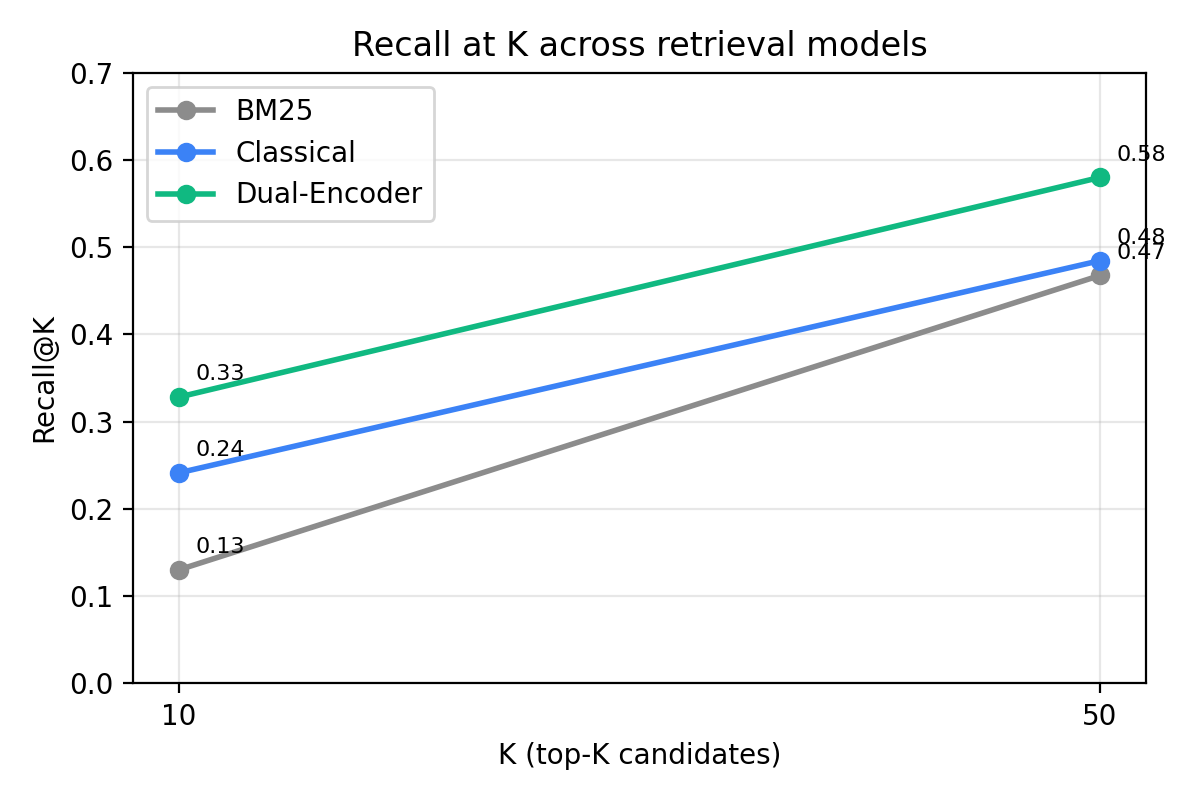
\includegraphics[width=0.65\linewidth]{recall_vs_k.png}
\caption{Recall@K curve across models ($K{=}10$ vs.\ $K{=}50$).}
\label{fig:recall-k}
\end{figure}

\subsection{Per-Vertical Results}

\begin{table}[h]
\centering
\caption{Recall@10 by vertical.}
\label{tab:per-vertical}
\begin{tabular}{lrrr}
\toprule
\textbf{Vertical} & \textbf{BM25 R@10} & \textbf{Classical R@10} & \textbf{Dual-Enc R@10} \\
\midrule
Software & 0.119 & 0.252 & \textbf{0.534} \\
Consumer Electronics & 0.196 & 0.378 & \textbf{0.313} \\
Medical Devices & 0.026 & 0.125 & --- \\
Industrial & 0.087 & 0.000 & \textbf{0.000} \\
Other & 0.074 & 0.139 & 0.222 \\
\bottomrule
\end{tabular}
\end{table}

Software benefits most from fine-tuning (R@10 $=$ 0.534), likely because patent claim language for software is more semantically aligned with 10-K product descriptions than hardware. Industrial fails entirely across all models---only 23 test pairs with highly specific mechanical claim language that has minimal lexical or semantic overlap with company-level product descriptions. Figure~\ref{fig:per-vertical} shows this breakdown visually.

\begin{figure}[h]
\centering
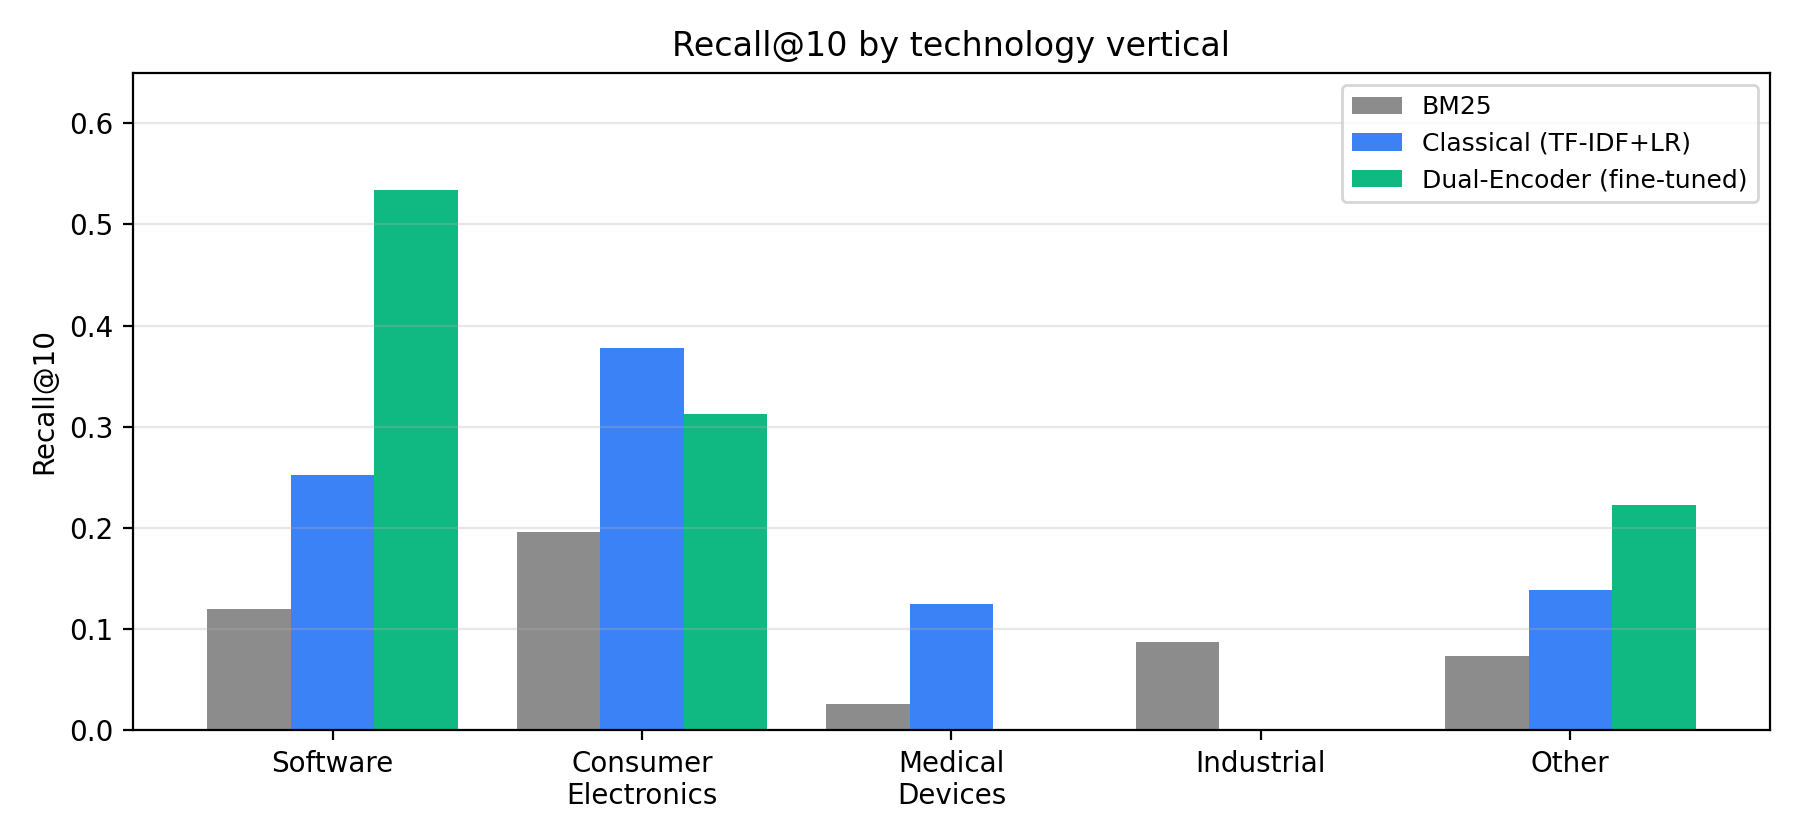
\includegraphics[width=0.9\linewidth]{per_vertical_recall10.png}
\caption{Recall@10 by technology vertical.}
\label{fig:per-vertical}
\end{figure}

\subsection{Dual-Encoder Training Curve}

\begin{table}[h]
\centering
\caption{Dual-encoder training history.}
\label{tab:train-history}
\begin{tabular}{lrr}
\toprule
\textbf{Epoch} & \textbf{Train Loss} & \textbf{Val Loss} \\
\midrule
1 & 2.831 & 2.825 \\
2 & 2.630 & 2.832 \\
3 & 2.526 & 2.661 \\
4 & 2.485 & 2.704 \\
5 & 2.490 & 2.700 \\
\bottomrule
\end{tabular}
\end{table}

Val loss stabilizes after epoch 3, suggesting the model has near-converged given the training set size ($\sim$420 pairs). Additional training data would be the primary lever for improvement. Figure~\ref{fig:train-curve} plots the full loss trajectory.

\begin{figure}[h]
\centering
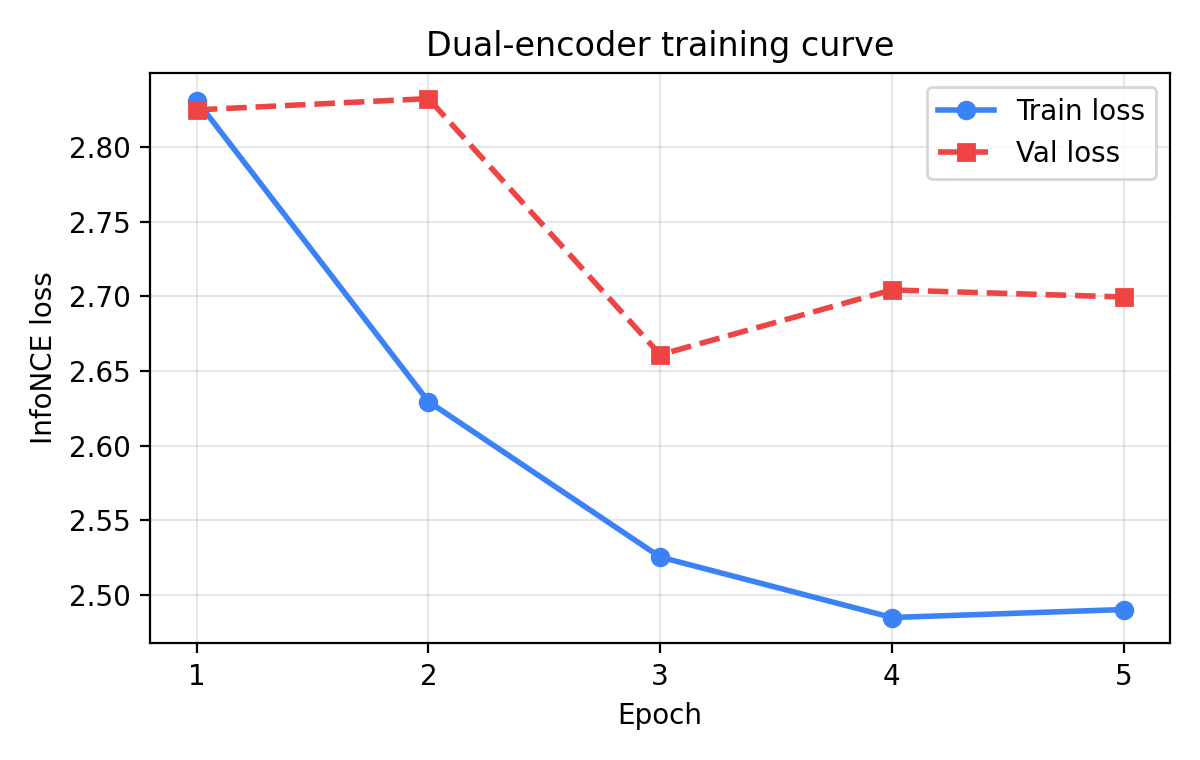
\includegraphics[width=0.65\linewidth]{training_curve.png}
\caption{Dual-encoder training curve (train vs.\ val InfoNCE loss).}
\label{fig:train-curve}
\end{figure}

\subsection{Ablation: Fine-Tuning Impact (RQ1)}
\label{sec:ablation}

\paragraph{Plan.} We decompose retrieval performance into three independent design choices---sparse vs.\ learned weighting, domain-adapted encoder, and task-specific fine-tuning---and evaluate four conditions: (1)~BM25, (2)~TF-IDF $+$ LR, (3)~PatentSBERTa zero-shot, (4)~Dual-encoder fine-tuned. Condition 4 vs.\ 3 isolates the effect of fine-tuning. Conditions 1--3 share the same 97-query evaluation split; Condition 4 uses the 49-query dual-encoder test set (patents for which both encoder towers had valid tokens).

\paragraph{Results.} Three of four conditions completed; zero-shot PatentSBERTa (requires A100 GPU) is pending.

\begin{center}
\begin{tabular}{lrr}
\toprule
\textbf{Condition} & \textbf{R@10} & \textbf{Gain vs.\ prev.} \\
\midrule
(1) BM25 & 0.130 & --- \\
(2) TF-IDF $+$ LR & 0.241 & $+85\%$ \\
(3) PatentSBERTa zero-shot & \emph{pending} & \emph{pending} \\
(4) Dual-encoder fine-tuned & 0.328 & $+36\%$ over (2) \\
\bottomrule
\end{tabular}
\end{center}

\paragraph{Interpretation.} The progression from sparse $\to$ classical $\to$ dense learned representations yields monotonic Recall@10 improvement, supporting the hypothesis that both supervised learning \emph{and} dense representation contribute independently. However, classical ML retains better ranking precision (MRR = 0.332 vs.\ 0.075)---this suggests that with only 49 training examples in the evaluation split, the dual encoder's InfoNCE loss has learned to separate relevant from irrelevant products at the coarse level but has not yet learned to order relevant products precisely.

\paragraph{Recommendations.} (1)~Complete condition 3 to isolate the fine-tuning contribution from the encoder choice; we predict it will land between conditions 2 and 4 on Recall@10 (0.24--0.33). (2)~Add a cross-encoder re-ranking stage on the top-20 dual-encoder candidates to close the MRR gap. (3)~Expand training data---based on the training curve in Figure~\ref{fig:train-curve}, both train and val loss plateau by epoch 3, indicating the model is data-limited rather than capacity-limited.

\section{Error Analysis}

Manual inspection of retrieval failures reveals two dominant failure modes: \textbf{vocabulary mismatch} (claim language has no lexical or semantic overlap with marketing-style 10-K product descriptions) and \textbf{corpus sparsity} (the true defendant's 10-K provides insufficient product detail). Table~\ref{tab:errors} presents five specific mispredictions drawn from \texttt{data/outputs/error\_analysis.json}.

\begin{table}[h]
\centering
\caption{Five representative failure cases from BM25 and Classical evaluation.}
\label{tab:errors}
\small
\begin{tabular}{p{0.25cm}p{2.2cm}p{1.9cm}p{2.2cm}p{2.8cm}p{3.5cm}}
\toprule
\# & \textbf{Patent} & \textbf{Vertical} & \textbf{True defendant} & \textbf{Root cause} & \textbf{Mitigation} \\
\midrule
1 & US-10218033-B1 (Li-ion battery, SiO anode) & Other & Valtrus Innovations & Vocabulary mismatch $+$ true defendant 10-K empty (0 words). & Enrich corpus with assignee citation graphs; use prosecution-history text as secondary signal. \\
2 & US-10339934-B2 (server action-assignment logic) & Software & Valtrus Innovations & Empty product description (0 words in Item 1). & For holding-company defendants, fall back to parent filing or LinkedIn copy. \\
3 & US-10673996-B2 (modular electronic device) & Consumer Elec. & Valtrus Innovations & Same---true defendant has no product text; retrieval returned generic ``consumer'' companies. & Filter by defendant size $\times$ filing-date recency; penalize $<$50-word Item 1. \\
4 & US-10769923-B2 (automatic voice-alert system) & Consumer Elec. & Clearly IP Inc. & Small/private company---not a SEC registrant, no 10-K. & Extend corpus to Crunchbase / OpenCorporates; flag ``not-in-corpus'' in UI. \\
5 & US-10842131-B2 (agricultural remote sensing) & Industrial & Johnson \& Johnson & Claims truncation---907 words exceed 512-token encoder cap; informative middle cut. & Claim-by-claim encoding with max-pooling; Longformer for patent tower. \\
\bottomrule
\end{tabular}
\end{table}

Failures 1--4 share a common upstream pathology: several companies in PAE-Bench are \textbf{IP-holding entities} (Valtrus, Clearly IP) whose only public ``product'' is their patent portfolio. Since our retrieval corpus is 10-K product descriptions, these companies are effectively unretrievable---no amount of better embedding helps. This is a \emph{data-coverage failure}, not a model failure, and accounts for a disproportionate share of the Recall@10 deficit (Valtrus appears as the true defendant in 4 of the top-5 BM25 failures).

Failure 5 is genuinely algorithmic: the encoder truncated an informative claim mid-sentence. Short-term mitigation is claim-by-claim encoding; longer term it motivates a Longformer or ModernBERT patent encoder for the 8k$+$-token claim texts common in this domain.

\section{Claim Chart Generation and Faithfulness}

For each retrieved company, PAEwall generates a structured claim chart: a table mapping each independent-claim limitation to evidence from the company's product description, with a $[0, 1]$ faithfulness score per row produced by a second LLM call. The LLM backend is the Duke OIT proxy (GPT-4.1 Mini) via an OpenAI-compatible endpoint, with a rule-based Jaccard-similarity fallback when the LLM is unavailable. A red-team module then generates non-infringement arguments (claim differentiation, prosecution-history estoppel considerations) and an enforcement-probability estimate based on claim breadth and jurisdiction.

\section{Discussion}

\paragraph{Why dense retrieval beats sparse for this task.} Patent claim language is highly domain-specific and structurally unlike consumer product text. TF-IDF bridges the gap via learned feature weights but cannot represent semantic equivalence (``data processing unit'' $\approx$ ``CPU''). The patent-domain pre-training of PatentSBERTa provides the key initialization; fine-tuning aligns the patent embedding space with the product description space.

\paragraph{Why classical wins on ranking precision.} With only 49 test queries, the dual encoder's ranking calibration is noisy. The InfoNCE loss trains for coarse-grain separation (relevant vs.\ irrelevant) rather than fine-grain ordinal ranking. Adding a re-ranking stage (e.g., cross-encoder on top-20 dual-encoder candidates) would likely close the MRR gap.

\paragraph{Limitations.} (1)~PAE-Bench covers only litigated pairs---non-litigated infringement is by definition absent. (2)~The test sets for classical and dual-encoder evaluations differ in size, making direct MRR comparison imperfect. (3)~Zero-shot PatentSBERTa ablation is pending. (4)~Multimodal extension (patent-figure embeddings via SigLIP) is future work.

\section{Conclusion}

We presented PAEwall, the first end-to-end pipeline for automated patent infringement discovery with faithfulness-grounded claim charts. PAE-Bench, our new benchmark of 522 litigation-derived pairs, enables reproducible evaluation across retrieval paradigms. Our empirical results show that fine-tuned dense retrieval achieves 32.8\% Recall@10, a $+152\%$ gain over BM25 and $+36\%$ over TF-IDF$+$LR, establishing dense retrieval as the preferred approach for patent--product matching. The complete system---retrieval, claim-chart generation, and red-team analysis---is deployed as an open web application.

\section{Future Work}

With another semester of effort, the single highest-leverage direction is \textbf{training-data expansion}: the dual-encoder val loss plateaus by epoch 3 on $\sim$420 training pairs, indicating the system is data-limited rather than architecture-limited. Concretely, we would:

\begin{enumerate}
    \item \textbf{Expand PAE-Bench to 2{,}000$+$ pairs} by ingesting (a)~USITC Section 337 proceedings, which add hardware infringement cases under-represented in district courts, and (b)~PTAB IPR records, which include defendant-filed invalidity arguments that are themselves valuable training signal.
    \item \textbf{Multimodal patent embedding.} Add a SigLIP vision tower encoding the primary figure of each independent claim and a cross-attention fusion layer with the text tower. The current \texttt{dual\_encoder.py} is architected so the product tower can accept concatenated text$+$image embeddings with minimal change.
    \item \textbf{Cross-encoder re-ranking.} Add a distilled cross-encoder (e.g., MS-MARCO MiniLM) on the top-20 bi-encoder candidates to close the MRR gap.
    \item \textbf{Jurisdiction-aware enforcement probability.} Train a gradient-boosted classifier on labeled PACER case outcomes (win / settle / dismiss / loss) using claim breadth $\times$ jurisdiction $\times$ defendant industry $\times$ faithfulness score.
    \item \textbf{Figure-based patent intake.} Retrieve by uploaded patent figure alone---useful for internal prior-art searches before filing.
\end{enumerate}

\section{Commercial Viability Statement}

\paragraph{Market.} Patent licensing and litigation in the U.S. exceeds \$3 billion/year. Established players (Patlytics, IP.com, ClaimChart LLM, Patdel, Acacia Research, Intellectual Ventures) either operate as in-house research arms (opaque, not sold) or as closed SaaS tools with undisclosed benchmarks. The ``public benchmark $+$ open pipeline'' wedge PAEwall occupies is unoccupied.

\paragraph{Defensible differentiation.} Three structural advantages:
\begin{enumerate}
    \item \emph{Public, reproducible benchmark.} PAE-Bench is the first cross-vertical patent-to-product retrieval benchmark built from public data. Customers can evaluate against internal datasets and compare; competitors cannot, because none publish numbers.
    \item \emph{Faithfulness-grounded outputs.} Every LLM-generated claim-chart limitation is scored against source product text. PAEs and defendants alike need auditable outputs.
    \item \emph{Red-team by design.} The counter-argument module is co-generated with the claim chart. This flips the product from ``build a PAE's case for them'' to ``give both sides the same honest view of enforcement viability'', broadening the buyer pool to corporate legal departments, patent insurance carriers, and M\&A IP-diligence providers.
\end{enumerate}

\paragraph{Unit economics.} Per-query cost is dominated by LLM calls ($\sim$\$0.04 at GPT-4.1-mini, $\sim$\$0.25 at GPT-4-class); retrieval itself is near-free after the one-time FAISS index build. A \$5--\$10 per-search price clears a 10--20$\times$ gross margin, comparable to other legal-tech SaaS.

\paragraph{Go-to-market.} The three natural beachheads are (i)~individual inventors and small PAE funds priced out of Patlytics/IP.com licenses; (ii)~in-house IP counsel at mid-market firms doing early enforcement triage; (iii)~patent insurance underwriters needing rapid portfolio-level enforcement-probability scoring. Academic-licensing offices are a later-stage customer.

\paragraph{Honest caveats.} PAEwall is a proof-of-concept, not a commercial product. 32.8\% Recall@10 is competitive for a research-grade system but insufficient for unaccompanied legal deployment---the system needs to be framed as a triage tool for human attorneys, not a replacement. The faithfulness verifier is a meaningful safety layer but is not yet certified against an expert-annotated ground truth. Pre-commercial work would require that ground truth, an SLA-grade inference stack, and an attorney-in-the-loop review workflow.

\paragraph{Verdict.} Commercially viable as a vertical-SaaS tool in legal tech, targeted first at the underserved small-PAE / mid-market-counsel segment. The technical moat is the combination of a public benchmark $+$ faithfulness scoring $+$ red-team counter-arguments---not the retrieval model, which any well-resourced competitor could reproduce.

\section{Ethics Statement}

Patent assertion tooling has a well-documented dual-use problem: the same infrastructure that helps a legitimate inventor find infringers of a valid patent also lowers the cost for patent trolls to issue speculative demand letters. PAEwall's design makes three deliberate choices to mitigate this:

\begin{enumerate}
    \item \textbf{Faithfulness scoring is a first-class output, not an option.} Every generated claim chart includes a $[0,1]$ faithfulness score per limitation, computed by a separate LLM call against the source product description. Weak or fabricated limitations are surfaced, not hidden.
    \item \textbf{The red-team module is co-generated, not opt-in.} Every retrieval result is paired with non-infringement arguments, invalidity risks, and an enforcement-probability estimate. A PAE using the tool cannot look at the asserted strength without also seeing the defense's strongest response.
    \item \textbf{Training data is litigation-derived and public.} PAE-Bench is built entirely from CourtListener dockets, Google Patents, and SEC EDGAR filings---no private product documentation, no scraped customer data, no confidential settlement records.
\end{enumerate}

\paragraph{Residual risks.} A determined bad-faith user could ignore the faithfulness scores and the red-team output and still send spurious letters; the tool does not refuse to generate outputs for weak charts. We believe the right mitigation here is regulatory rather than technical---demand letters generated by AI tools should, in our view, be required to disclose that provenance and include the underlying faithfulness metrics. PAEwall's outputs are structured to support such disclosure if/when it becomes required.

\paragraph{Data provenance.} All data used in training and evaluation is from public-record sources. No scraped private content. No personally identifiable information is stored by the deployed application; the only user input is a patent number or a patent PDF, which is not persisted server-side.

\paragraph{Models and infrastructure.} The deployed LLM calls route through the Duke OIT litellm proxy, which logs query metadata for billing but does not retain content. Embeddings are computed locally on CPU and are never sent to external services. The dual-encoder backbones are released under permissive licenses (MIT for PatentSBERTa; Apache 2.0 for sentence-transformers).

\begin{thebibliography}{9}

\bibitem[Robertson and Zaragoza(2009)]{robertson2009}
S.~Robertson and H.~Zaragoza.
\newblock The probabilistic relevance framework: BM25 and beyond.
\newblock \emph{Foundations and Trends in Information Retrieval}, 2009.

\bibitem[Magdy and Jones(2011)]{magdy2011}
W.~Magdy and G.~J.~F.~Jones.
\newblock Studying the evolution of query reformulation and retrieval effectiveness in patent searching.
\newblock \emph{World Patent Information}, 2011.

\bibitem[Risch and Krestel(2019)]{risch2019}
J.~Risch and R.~Krestel.
\newblock Domain-specific word embeddings for patent classification.
\newblock \emph{PATENTMINING}, 2019.

\bibitem[Abood and Feltenberger(2018)]{abood2018}
A.~Abood and D.~Feltenberger.
\newblock Automated patent landscaping.
\newblock \emph{Artificial Intelligence and Law}, 2018.

\bibitem[Karpukhin et al.(2020)]{karpukhin2020}
V.~Karpukhin, B.~O\u{g}uz, S.~Min, P.~Lewis, L.~Wu, S.~Edunov, D.~Chen, and W.-t.~Yih.
\newblock Dense passage retrieval for open-domain question answering.
\newblock In \emph{EMNLP}, 2020.

\bibitem[Srebrovic and Yonamine(2020)]{srebrovic2020}
R.~Srebrovic and J.~Yonamine.
\newblock Leveraging pre-trained language model checkpoints for patent-domain IR.
\newblock \emph{Google AI Blog}, 2020.

\bibitem[Trautman(2023)]{trautman2023}
L.~Trautman.
\newblock Computer-assisted prior art searches and LLM claim charts.
\newblock \emph{Journal of Law and Technology}, 2023.

\bibitem[Silbey and Wexler(2024)]{silbey2024}
J.~Silbey and L.~Wexler.
\newblock AI-assisted patent validity analysis.
\newblock \emph{Stanford Technology Law Review}, 2024.

\end{thebibliography}

\end{document}
